\documentclass[11pt]{article}
%Gummi|065|=)
\usepackage[linesnumbered,ruled,vlined]{algorithm2e}
\usepackage{xcolor}
\usepackage[utf8]{inputenc}
\usepackage{amsmath}
\usepackage{amssymb}
\usepackage{changepage}
\usepackage{graphicx}
\usepackage{hyperref}
\usepackage{listings}
\usepackage{xcolor}
\usepackage[english]{babel}
\usepackage{titlesec}
\definecolor{codegreen}{rgb}{0,0.6,0}
\definecolor{codegray}{rgb}{0.5,0.5,0.5}
\definecolor{codepurple}{rgb}{0.58,0,0.82}
\definecolor{backcolour}{rgb}{0.95,0.95,0.92}

\lstdefinestyle{mystyle}{
    backgroundcolor=\color{backcolour},   
    commentstyle=\color{codegreen},
    keywordstyle=\color{magenta},
    numberstyle=\tiny\color{codegray},
    stringstyle=\color{codepurple},
    basicstyle=\ttfamily\footnotesize,
    breakatwhitespace=false,         
    breaklines=true,                 
    captionpos=b,                    
    keepspaces=true,                 
    numbers=left,                    
    numbersep=5pt,                  
    showspaces=false,                
    showstringspaces=false,
    showtabs=false,                  
    tabsize=2
}

\lstset{style=mystyle}
\title{\textbf{Internship report}}
\author{Nicolas YAX}
\date{}
\begin{document}

% BIG ISSUE:
% You need to focus more on what you did. There are pages and pages of unrelated stuff before we even learn about what you did! I know that you need to give some context, but this is way to much. Many sections are just a distraction in my opinion, and hide the true goal of your work. For example:
% - regularization loss term. why is this relevant?
% -  supervised learning
% - details about RL & PPO. We just need to know the basics, and that PPO is the state of the art method for our kind of problem. No need to expand like crazy.
%  Either remove or put in an appendix. 
% You really need to have a clearer story to tell:






% OTHER IMPORTANT REMARK: are you expected to have citations? if so, you need to cite people each time you explain something that you didn't do yourself.

\maketitle
M1 student - ENS Paris Saclay - Adrien Doerig - Tim Kietzmann

NOTE : \underline{words underlined} are defined in appendix if needed.
\section{General view of the project}
% 1. What is the project about and why is it interesting? -> vision in general in bio+ artificial systems, saccades, etc. why saccades are important.
% I've tried to summarize your grant intro very quickly
In last few years Deep Neural Networks (DNNs) have become a major tool in computer vision. They have been used both to solve engineering issues such as face recognition as well as brain modelisation. However this modelization lacks several crucial aspects of biological neural computation but this is an open question.

\underline{Oracles} in computer vision are mostly human based which means trying to bridge the gap could improve both engineering and neuroscience modelizations. We have found two main differences that could be investigated :
\begin{itemize}
\item DNNs are mostly feed forward where brain computation is heavily based on recurrences which makes it possible to integrate information through time.

\item DNNs see images globally where humans only focus on small parts and saccades to progressively integrate the whole image
\end{itemize}

Those two observations combined together might truely improve the efficiency of DNNs used for computer vision.

Thus our work will focus on building a system that can classify images only by seeing small crops of them and by saccading and integrating information through time.

\subsection{Lab context}
For this internship I'm working with Adrien Doerig (Postdoc researcher - Internship supervisor) and Tim Kietzmann (Assistant Professor - Team supervisor). This team has been created in September 2019.
This is a new project (I'm the first one with Adrien to work on it) and it will be continued for a few years. My job will then be to start this project by creating tools for the next ones to work on it and to get first results with a simple version of our original pipeline.

\section{Approach}
% 2. Which approach did you take? -> making artificial systems more bio plausible by adding eye movements, which has never been done before. How? -> coupling reinforcement learning to learn where to look with recurrent CNNs to integrate info over time and classify images based on sequences of saccades.
Our goal is to make artificial systems more bio plausible by adding eye movements. This is an original idea that has never been tried on this scale before. The only work with using saccades we have found was from Mnih and Al (2015) where they have trained a recurrent system to learn on \underline{MNIST dataset} with a very simple system using a basic reinforcement learning algorithm. The system was provided 3 crops with different zooms to classify images which is too far from human vision for us.

Our idea is to go further than this and to train more bio close system with only one crop (and not 3 with different zooms) with state of the art recurrent neural networks developped by the lab, state of the art reinforcement learning algorithms and we will try to scale it to more realistic data.

Our pipeline will be based on reinforcement learning to teach the neural network where to look in the image and standard supervised learning algorithms to learn how to integrate information through time. This should result in a classifier/saccader system which classifies images as sequences of crops and makes it a very original interaction between 2 sides of machine learning that usually never cross.

This interaction is so special that most reinforcement learning framework aren't optimized for it. My job will firstly focus on how to hack those frameworks from outside to implement such a pipeline and then implement my own framework to make it easier for the others to implement their experiments. Secondly I'll use this new framework to get first results about a simple version of the pipeline.

Due to the corona crisis I had to run everything on my own computer which means I mainly focused on a very modest system, small and simple images and few neurons. In this second part, my job was to try to get results as close to Mnih and Al paper as possible with only one crop and a state of the art reinforcement learning algorithm.

\section{Prerequisite knowledge}
% 3. Prerequisite knowledge. Explain what people need to know. DON'T LINGER ON UNRELATED DETAILS -> direct people to the appendix if you really want to include details. You should explain in simple words what the principles are (e.g. Reinforcement learning is a family of methods to learn by interacting with the world - and expand a bit but not too much). Then, say that mathematical details are in the appendix. What is important is that your reader understands what you are doing, not that they know all equations. At the moment, I don't understand what you are doing, and I just get lost in equations that you don't even have time to explain thoroughly.
As explained before we used reinforcement learning and recurrent neural networks. These notions will be briefly explained in next paragraphes in order to give the overall idea about what these things are. If you need more details about math there are further explanations in appendices.

\subsection{Reinforcement Learning}
\begin{figure}[!h]
\centering
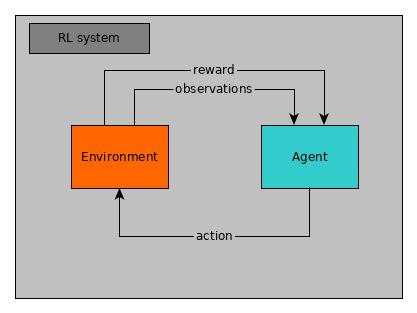
\includegraphics[scale=0.40]{rl.jpg}
\caption{RL system : the agent will see its environment (collect observations) and learn to react to it (chose action) in order to get the highest cumulated reward}
\label{rl}
\end{figure} 
This part of machine learning involves involves an agent / environment system where the agent will have to learn to behave in order to maximize a reward \ref{rl} .

Reinforcement learning is a \emph{Markow Decision Process}, the environment has states observed by the agent and transitions are trigered by actions from the agent. Each transition returns a reward that will be sent to the agent which will try to maximize its total reward over a run.

Initially the agent doesn't know the environment and will try after several trajectories in the environment to understand it and to optimize its behaviour in order to find best paths to get the best reward possible.

Behaviour of the agent (function that from an observation returns the action) is called its \textit{\underline{policy}}.

% details not needed in main text
\paragraph{Policy Gradient and REINFORCE}
The philosophy of policy gradient methods is to see the policy as a function that will be directly learnt by a neural network. The algorithm will proceed in 2 phases : collecting batches of trajectories and fitting the policy to learn the best way to optimize rewards. To optimize it it will compute a loss function and apply a gradient descent on it through the neural network. REINFORCE is the direct implementation of this philosophy.

% details not needed in main text
\paragraph{PPO}
PPO is a state of the art Policy Gradient algorithm designed by OPENAI. It aims at improving REINFORCE by adding few features in the loss function. First when using an algorithm such as REINFORCE, the policy might change too much when fitting. Let's assume the environment is divided into several phases (summer,automn,winter,spring for example) where results of actions could be very different from a phase to another. This kind of learning might result in a policy that would change too much and \underline{overfit} on each phase, forgetting everything learnt during the previous phase. There is no perfect solution for this issue.

PPO adds a term in the loss that will try to not move too much from the previous policy in order to avoid such a behaviour.
% why is this here? computer vision and CNNs would make more sense right after the part on ANNs. here is seems like you are going back and forth between unrelated topics.
\subsection{Computer Vision}
The main problem addressed in computer vision in which we will be interested is the classification problem. Given an image representing something among a set of defined classes (such as [cats,dogs]), the algorithm needs to find the right class in which the image belongs. This means it has to integrate what is represented in the image to classify and label it correctly. Actual methods used to solve this problem strongly relies on neural networks.

\paragraph{Convolutional Neural Networks}
Convolutional neural networks are inspired by the internal structure of visual areas (LGN,V1,...) in brain. It makes it possible to compute images very efficiently. It's easier to understand convolutional neural networks by seeing states of layers as images (2 or 3D arrays). They make it possible to process images more properly with more adapted data structures. Convolutional neural networks have less parameters than traditional networks and an invariance to translation which results in better internal representation of what it's learning.

\subsection{Recurrent Neural Networks}
A recurrent neural network works similarly than a simple neural network excepts that it will keep an internal state that will be updated after each call to the model and interfer with next calls. This means it will be able to integrate information thought time with this recurrent state and learn how to encode data in its state and how to decode it.

% shouldn't this come earlier?
\section{Detailed approach}
% 4. Detailed approach / methods: what exactly did you try, and how did you implement it? What problems did you face and how did you change your approach to solve them? You can explain here that you tried two things: OPENAI and RLLIB.
This part will be separated in 2 subparts : first we will examine different structure used to train both networks and results got for each structure. Then we'll take a look at the framework I have designed and developed in order to see which tools I have been using and how I've implemented them.

% IMPORTANT: you need to explain the idea behind the framework, with two networks interacting - one rCNN and one RL network. explain that the RL learns where to look based on activity in one of the rCNN layers, explain why this makes sense, etc... This is a CRUCIAL part of the project (everything is based on it), so give it a predominant place!

\subsection{Contribution - Structure of the system}
The main idea is to combine 2 networks : a recurrent classifier that would see crops and try to guess the label and a saccader that would understand where to crop for the classifier to classify the crop correctly.

\paragraph{Classifier}
The classifier will take crops as input (9x9 grayscale images) - Mnih used 8x8 crops but 9x9 crops have a better semantics as they are centered on a pixel. It will then process it through several layers. My best results weren't with convolutions but with classic recurrent layers because MNIST is very simple and is more efficient to learn on it with simple layers. Obvisouly to scale the pipeline to realistic images, convolution would be a must have. The output is an array of size 10 because there are 10 classes in MNIST. Each scalar reprensents the probability for crops processed to represent the class of the scalar's index in the array. Be carefull, sum of the array isn't one, if an image reprensenting a mix between 2 digits is given to the network it might return one for each of those classes. The predicted label will be the index with the maximum returned probability.

 It then possible to compute how much the network is sure about its prediction by computing the \underline{crossentropy} of the output for the given label. If it's close to 0 it means the network is very sure about its prediction (entropy of zero means one for the predicted label - and it's the right one - and 0 for the others). Thus if an image representing a mix between 2 classes is fed to the classifier and it returns a huge probability for both classes, the \underline{crossentropy} would be very high.
\paragraph{Saccader}
We want the saccader to understand where to crop for the classifier to be able to classify correctly. Thus it might be a good idea for the saccader to not have the crop as input but an internal layer of the classifier. Thus it should be able to understand the actual state of the classifier and to return the right crop to complete information held by the classifier. For my internship the saccader isn't recurrent, only the saccader is. The output of the saccader is a vector of size 2 representing x and y normalised coordinates for the next crop. The saccader will learn with PPO which means we need to define a reward and that's where there are many possibilities :
\begin{enumerate}
\item Issue each iteration (reward of 1 if the prediction is right each time the classifier is called, 0 else)
\item Issue at the end (reward of 1 only at the end of the loop if the final prediction is right, 0 for the other iterations and if it's wrong)
\item Minus crossentropy each iteration (the crossentropy is the loss of the classifier for its prediction - it represents how much the classifier is sure about its prediction and about the fact that prediction is right)
\item Inverse crossentropy (a custom reward begin equal to $tanh(\frac{1}{crossentropy})$). The main reason behind this is that when the crossentropy is very close to 0, the network is very sure about its prediction and that's a thing we should encourage. This means by increasing the reward, the saccader will try to look at positions which will confort the classifier in its prediction. Thus taking the inverse of the crossentropy is super relevant as it will limit noise about not sure predictions and it will highly increase the reward for sure positions. Finally after a long training, the classifier should be pretty sure about its predictions which means the reward might be too high. Clipping it with a tanh is a solution to avoid having insane rewards.
\end{enumerate}
We have tested each of them.
\paragraph{System}
Once the classifier and the saccader are computed here is how the whole pipeline works :
\begin{enumerate}
\item For each image, an initial crop which is centered (coordinates [0.5,0.5]) is computed. 

\item The crop is then given to the classifier that will try to classify it (but at this stage its probability to be correct is low) and will compute the input for the saccader (internal layer of the classifier). The classifier can then compute new position for the crop and the new crop will be computed. If 6 crops have already been computed it stops, else it jumps to 2.
\end{enumerate}
We have chosen to take 5 saccades (6 crops) as it's not a lot (efficient to compute quickly) but still far enough to classify correctly each digit (Mnih and Al used up to 8 crops).

Once several images have been treated, both networks will fit on these data : the classifier will backprop on its loss : a \underline{sparse\_categorical\_crossentropy} loss function using crops it got as input, its predicted label and the real label. The saccader will keep track of its trajectories : observation/action/reward computed during trajectories. It will then backprop on the PPO loss to optimize the policy. Those trainings are done at the same time to have a better synchronisation between both networks.
\subparagraph{Chaotic system}
This classifier + saccader learning system is very unstable : let's assume the saccader one saccades on the top left hand corner. The classifier will only get crops from this fixation. This means it will fit on top left centered crops and won't develop knowledge about the rest of image space. If it only sees the top left part of digits when it sees an other crop it won't understand it and won't be able to classify it. This way when the saccader explores, crops won't be understood by the classifier which will result in low rewards. Thus the system will be stuck on the top left spot and won't move anymore event if this spot isn't optimal. This means the function that is minimized through this process has a lot of local minima and the starting point and the way optimization is done are crucial. This makes the system very unstable which is akward because usually supervised learning of classifiers is very reliable.

\subsection{Contribution - Framework}
As the first one to actively work on the project, my job is to create a reliable framework for the next ones to work on the project to easily implement new things. They should worry about learning all frameworks used to handle the RL part and the supervised part. My goal is thus to create an easy to learn, easy to understand and easily expandable framework that can hide hacks of RL frameworks and handle them for the user without them having to understand how they work.

RL frameworks we have used are recent which means the documentation is very soft and it's often hard to find why your program doesn't work with information found in the documentation or on the internet. To understand how to implement such an innovative and original system I had to read the source code of huge libraries to produce a small code that would actually work fine. This lack of documentation was a real issue and I've spent most of my time reading and printing everything in RL frameworks to really understand how to hack those into our original system.


\subsubsection{GRLF - Graph Reinforcement Learning Framework}
% the following is not bad, BUT, it would be important to first provide an overview of what you are trying to achieve. maybe show an image with the structure of the framework, which shows the different modules and what their purpose is. then, you can explain in detail how it works, as you do in the following part here. 
% you should explain "here is what we want: [explain the idea of training two networks in synergy] and this is how we will implement it using modules [show an image of the final framework, and explain: the MNIST database module does X, the copper module does Y, etc.]. As you can see, this indeed does what we want: the modules work together to train both networks at the same time
It's fairly easy to draw the pipeline with a graph and its a versatile way to do it. It makes it possible to easily express the synergy between both networks and to efficiently modify the dynamics of the system only by moving few edges.
\begin{figure}[!h]
\centering
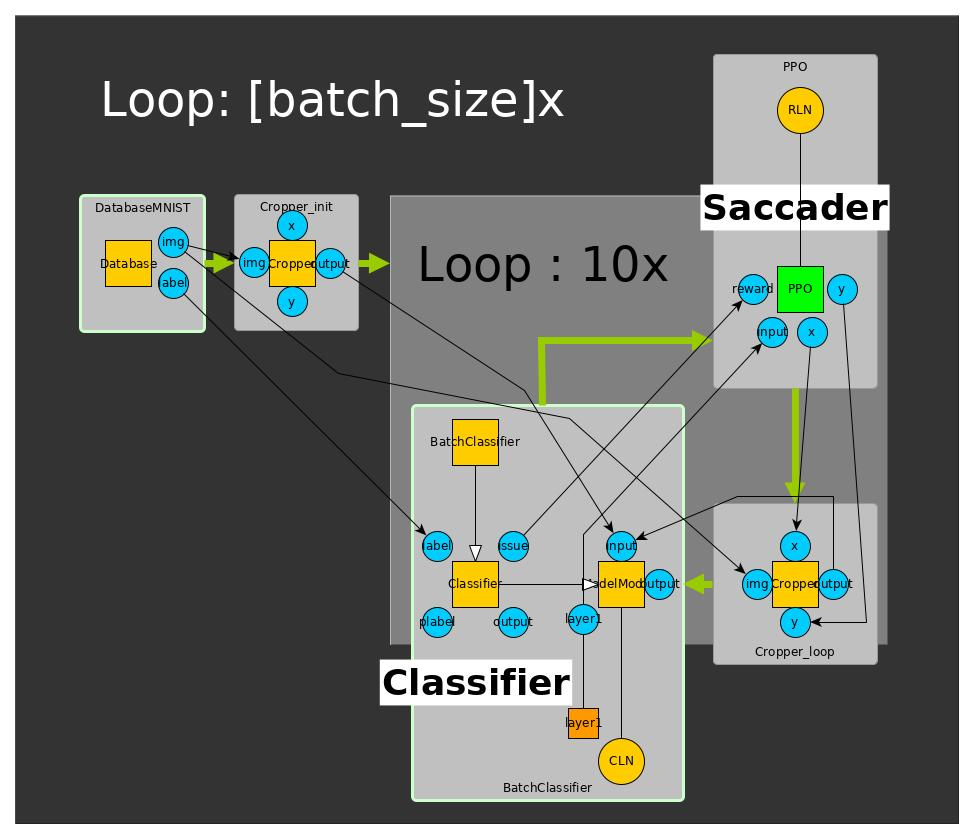
\includegraphics[scale=0.30]{design.jpg}
\caption{Graph design of the pipeline}
\label{design}
\end{figure}\\
That's why the framework I've designed is graph based. We want to write the pipeline we have discused before with a graph.

 You can find the same structure we have seen in previous subsection expressed as a graph \ref{design}. Database and initial crop are at the top left hand corner while the inner loop (loops 10x here) is on the right with the saccader, the classifier and a cropper to crop the image according the the saccader's outputs.

\paragraph{Aim of the framework}
To sum things up my main concern about making this framework is to
\begin{itemize}
\item Find a way to implement the original pipeline with both networks learning together using reinforcement learning librairies
\end{itemize}
Moreover my additional objectives about making this framework are to make it:
\begin{enumerate}
\item Easy to understand (learn and read code from others)
\item Easy to extend (everyone can add code)
\item Change the RL framework easily (versatile)
\end{enumerate}
Thus we will first see the structure of RL frameworks and why reinforcement learning librairies aren't made for this kind of applications and how I've came up with a way to make it work and then how I've designed the framework to implement these hacks.



\subsubsection{Structure of RL framework}
During this internship I have worked with 2 RL frameworks : OPENAI baselines (creators of PPO) and RLLIB (more scalable than OPENAI) but what we will see in next paragraphs apply on most RL frameworks.
Most RL framework uses the same global structure with 2 very different objects : Agents and Environments.
\paragraph{Environments}
Environments only provide observations and rewards. They are tools used by agents to learn. 
% they are not really tools, they are rather the world in which agents live & learn.
The most famous standard of environment is the gym environment (made by OPENAI) whose specification is fairly straightforward :
\begin{lstlisting}[language=Python]
class GymEnv:
	def __init__(self):
		#intializer
		self.observation_space = #type and shape of the observation space
		self.action_space = #type and shape of the action space
	def step(self,action):
		#modifies the state of the environment and returns obs,rew,done=(if the env needs to be reset),info=debug
		return next_observation,reward,done,info
	def reset(self):
		#resets the environment
		return initial_obs
\end{lstlisting}
This standard is widely used and all RL frameworks are compatible with this type of environment. RL frameworks have their own internal data structure for environments and have a function to convert gym environments into this representation. Usually when people give a gym environment for the training, the framework will create an internal environment that will represent an array of duplicated gym environments. This way the agent gets batches of observations and its more efficient to compute a batch of actions with neural networks and a GPU than actions one by one. Thus you cannot create a gym environment returning a batch of observations directly because the framework will considere the batch as a single observation. This means that in RL frameworks, Gym environments are strictly less expressive than the inner environment structure.

Because of the universal usage of Gym Environments it might be a good idea to use them especially because we want to switch RL framework easily (3). However they are less expressive than inner environment structure (that will change from a framework to an other) which might become an issue.
\paragraph{Agents}
In most RL frameworks, agents have the main loop during the training which means people call the train method of the agent and it will call the environment accordingly without any action from the user.

There isn't any universal standard for agents which means agents data reprensentations will change from a framework to an other. That's why we will need to be particularly careful to set a compatibility system so that any data structure from any RL framework is compatible with ours.

\subsubsection{Problems with a duo of networks}
% Probably just a detail -> remove ?
\paragraph{Batch system - OPENAI}
The RL part of the system is only the saccader. It's the only neural network that learn with RL when the classifier learns by supervised learning. This means our agent will have the saccader as neural network and the classifier will be part of the environment. However if we use gym environments, the framework will convert it to its own environment representation wy creating a batch of environments. We can make sure all these environments share the same classifier but it means that the inner environment will work with batches to make it possible for the saccader to learn faster. Thus the latter will return a batch of actions that will be distributed in each environment according to its index. The classifier will then be called by the enviroment on inputs one by one which is super inneficient. Thus it's not possible to efficiently use gym environments but we will need to sacrifice (3). For each framework we will need to create a conversion system to transform our graph based environment into the internal environment data representation for each framework used instead of just creating one for gym envionments.
%Probably just a detail -> remove ?
\paragraph{Branch network - RLLIB}
RLlib is more complex : it won't create a unique internal environment but several that will run on parallel workers (see it as computers in a network). This means the latter trick won't work especially because it's super hard to share the classifier between workers (tensorflow isn't made for that). This means we will have to put all our neural networks in the hub together. Both of them will be in the agent which can only have one neural network due to the agent structure TFPolicies in RLLIB. This means we will have to create a branched network that will take the standard input for the classifier and create outputs of both networks at once but only apply the RL algorithm on a single output. RLLib makes it possible for TFPolicies to define a custom loss function where we can cut the gradient of the RL loss on the classifier's outputs. Thus by adding a second term in the loss being the standard supervised loss for the classifier it's possible to train both networks at once with a gym environment (there isn't any network in the environment anymore).
\subsubsection{Structure of the framework}
Now that we have seen hacks I've been using to make it work let's see the structure of my framework to hide those hacks.
\paragraph{General system}
To be sure to be compatible with RL frameworks it's important to keep the agent/environment separation as it's the only common structure in all RL framework. The framework must make it possible for the user to define a system that will be compiled in an agent/environment system to call libraries accordingly. This way the user doesn't need to understand how RL framworks function in depth to build its system.
\paragraph{Graph dynamics}
The main idea is to propose an interface based on a graph which will be defined by the user describing the dynamics of the system \ref{graph_dynamics}. This graph will be composed of modules (nodes) that will be connected between each other.
\paragraph{Modules}
A module is an object that can be connected to other modules through its \emph{ports} (analogy with networks). A \emph{port} is a value from a module that can be accessed from other modules and shared with them. Basically a module gets information from other modules through its ports, computes something with thesd values and  stores outputs of the computation in its ports to be sent to other modules. Thus the following architecture will be used :
\begin{lstlisting}[language=Python]
class Module:
	def __init__(self):
		#intializer
	def run(self):
		#Compute things
\end{lstlisting}
Ports are defined using python objects as dictionaries : 3 prefix keys will be used to interact with ports :
\begin{itemize}
\item '*' : define a port and give its type
\item ':' : redefine the type
\item '$\epsilon$' : get the value of the port
\item '>' : used to create links between nodes (we will get back to this later)
\end{itemize}
Here is an example of the definition of a module :
\begin{lstlisting}[language=Python]
class DoubleModule:
	def __init__(self):
		#intializer
		self["*a"] = float #definition of port a as float
		self["*b"] = float #definition of port b as float
	def run(self):
		#Compute things
		self["b"] = self["a"]*2 #Use the value of port a to double it and put it in port b
d = DoubleModule()
print(d["a"])
>>> None
d["a"] = 5.
d.run()
print(d["b"])
>>> 10.
d[":a"] = int #Will autoconvert the initial value in a to int
d.run()
>>> Exception : port b has type float but received int value
d[":b"] = object #Universal type
d.run()
print(d["b"])
>>> 10
\end{lstlisting}
As you can see I've added a type system that doesn't exist in Python to make it more convenient for users. It's possible to bypass it if needed. Several modules can be defined this way to compute complex functions.
\paragraph{Connecting modules}
Modules can be connected with the following syntax :
\begin{lstlisting}[language=Python]
#Define module 1
module1 = Module()
module1["*a"] = int
#Define module 2
module2 = Module()
module2["*a"] = int
#Connect module1["a"] to module2["a"] (-> direction of arrows)
module1[">a"]([module2[">a"]])
\end{lstlisting}
\paragraph{Loop and Graph object}
Loop makes it possible to handle the system we have talked about to compute modules and ports dynamics :
\begin{lstlisting}[language=Python]
#Define module 1
loop = Loop([module1,module2],nb=1) #Modules will run in this order (nb=1 iteration of the loop)
module1["a"] = 5
print(module2["a"])
>>> None
loop.run() #run module1.run (empty) then send module1["a"] to module2["a"] and run module2.run() (empty)
print(module2["a"])
>>> 5
\end{lstlisting}
With this loop system it's possible to run a sequence of modules several times.
\paragraph{Graph and agent/environment system}
Graph object makes it possible to compute the agent/environment system. First we need to define a RL\_Module :
\begin{lstlisting}[language=Python]
import tensorflow as tf #Main ML library -> tf.Tensor is an array
class RL_Module(Module):
	def __init__(self,input_shape,output_shape):
		self["*input"] = (tf.Tensor,input_shape) #Observation : type and shape
		self["*output"] = (tf.Tensor,output_shape) #Action : type and shape
		self["*reward"] = (tf.Tensor,(None,1)) #Reward : type and shape
	def run(self):
		#Compute things
\end{lstlisting}
Once a RL\_Module is defined in a Loop object it can be upgraded to a Graph object in order to get the agent/environment system. This is a dummy example with empty modules to show how it works :
\begin{lstlisting}[language=Python]
#Definition of Modules (nodes)
rl_module = RL_Module((10,),(2,))
m1 = Module()
m1["*action"] = tf.Tensor
m1["*a"] = tf.Tensor
m2 = Module()
m2["*a"] = tf.Tensor
m2["*obs"] = tf.Tensor
m2["*reward"] = tf.Tensor
#Definition of connections
rl_module[">output"]([m1[">action"]])
m1[">a"]([m1[">a"]])
m2[">obs"]([rl_module[">input"]])
m2[">reward"]([rl_module[">reward"]])
#Definition of the graph
loop = Loop([m1,m2,rl_module],nb=10) #Run 10 times the list
graph = Graph(loop)
#Run the graph
print(graph.environment)
>>> GymEnv at XXXXXXXX
print(graph.agent)
>>> Agent at XXXXXXXX
graph.run(1000) #Run 1000 times the loop
\end{lstlisting}
It's then possible to only use the agent or the environment from the graph object with an other framework if needed. The agent is compatible with GymEnvironments and the environement is a GymEnvironment. You can also run both together with the graph.run method. We'll now see how to implement RL\_Modules more in depth to then go further in difficulties of implementation.
\paragraph{RL\_Modules more in depth}
In the team we aren't professionals of RL which means we will prioritize using existing powerful RL frameworks in order to be sure about the efficiency of the implementation of the algorithm. In most RL frameworks, agents are objects with a run method and an environment parameter. Calling this method will run the main training loop. However in GRLF the definition of the graph contains both the agent and the environment with a loop system including both. This means it's won't be easy to extract the environment and agent functions from this graph structure that include them both.

We have added a new method for modules : the run\_after method that will be called right after the run method. Now the RL\_Modules code looks like this :
\begin{lstlisting}[language=Python]
import tensorflow as tf #Main ML library -> tf.Tensor is an array
class RL_Module(Module):
	def __init__(self,input_shape,output_shape):
		self["*input"] = (tf.Tensor,input_shape) #Observation : type and shape
		self["*output"] = (tf.Tensor,output_shape) #Action : type and shape
		self["*reward"] = (tf.Tensor,(None,1)) #Reward : type and shape
		self.learn_fn = #Function from the RL framework : (env,nb_timesteps) -> object
	def run(self):
		#Compute things
		raise RLInput(self["input"]) #raises the exception
	def run_after(self):
		#Compute things with self["output"] = output of the agent in the RL framework
\end{lstlisting}

\subsubsection{Baseline modules}
% ALL OF THESE SHOULD COME UP IN THE BEGINNING OF THE FRAMEWORK. you should explain "here is what we want: [explain the idea of training two networks in synergy] and this is how we will implement it using modules [show an image of the final framework, and explain: the MNIST database module does X, the copper module does Y, etc.]. As you can see, this indeed does what we want: the modules work together to train both networks at the same time"
There are several objects modules can heritate from (which creates a type system over modules) : FitableModules (contains a datastructure that can learn) and PointerModules.
\paragraph{MNIST Database}
This module doesn't have any port used as input. It will fill its "img" port with a MNIST image and the "label" port with its label. Images and labels are changed each time the run method is called. Images are chosen in the order of the database (n call is the n-th image of the dataset).

\paragraph{Cropper}
This module is very simple : it gets as input an image "img" and crop coordinates "x","y" and the run method will return in "output" the smaller image corresponding to "img" cropped at those coordinates.

\paragraph{ModelModule - FitableModule}
A ModelModule has an internal neural network and two ports : "input", "output". Calling run calls the network on "input" and returns the result in "output". The user can also access any layer in the neural network through the port that has the same name.

\paragraph{Classifier - PointerModule FitableModule}
A Classifier module is a PointerModule to a FitableModule and will have 4 ports : a reshaped "output", a "label" port for the real label, a "plabel" port for the predicted label and a "issue" port with a boolean value about whether the predicted label is the same as the real label. Calling run will call the ModelModule run method, reshape the output to a given shape (it's more convenient this way), computes the predicted label from the output of the neural network to then fill the "issue" port.

\paragraph{BatchCapsule - PointerModule}
This pointer module is more complex : it will capture each input in "input" and "label" ports of the pointed module and store them in a batch. Once enough data collected (treshold defined by the user) it will fit the pointed module on collected data (it should point to a FitableModule).

\paragraph{PPOSaccader - PointerModule,FitableModule}
A RL\_Module with a learn\_fn for PPO which points toward a FitableModule. It will compute x and y coordinates for the saccade from the output of its FitableModule.

\paragraph{}
As you can see those modules makes it possible to train both networks and the framework stays pretty easy to use and to learn.

There are 2 different kind of RL frameworks : standard ones with simple execution and frameworks using workers to optimize the learning on GPU clusters. I've worked with both types of frameworks and developped a version of my own framework for each of these execution types.

\section{Results}
% 5. Results: show some of your results. here you can stress that this project is highly technical and challenging, and that your main contribution was to develop a way to do this. Nobody has ever done it before. Then, show some results that prove that what you developped works - i.e., show that the system learns (explain which baselines you used, etc.), contrast FF with recurrent networks and what they achieve, etc. You can split this up between the OPENAI and the RLLIB results in two different subsections.
I have tested 2 types of neural architecture :
\begin{itemize}
\item Feed Forward : the classifier isn't recurrent (easier to debug) which means the task of the saccader isn't to complete information the classifier needs to decide but to find the best spot for the classifier to classify with one crop.
\item Recurrent : classic pipeline.
\end{itemize}
Here are results after having seen 600 000 images (10 epochs) :
\begin{center} %I'm running things to fill it
   \begin{tabular}{| l | c || r | }
     \hline
      & Feed Forward & Recurrent \\ \hline
      baseline center &  & \\ \hline
      baseline random & & \\ \hline
      Binary reward & & \\ \hline
     Each step crossentropy reward & & \\ \hline
     End step crossentropy reward & & \\ \hline
     Custom crossentropy reward & & \\
     \hline
   \end{tabular}
 \end{center}
% I'll comment it

\section{Discussion}
% 6. Discussion: what works and what remains to be done
In the end, my goal has been achieved : the framework is done and respects most objectives and I've almost the same results speaking about accuracy than Mnih and Al. However if the training runs for too long, fixations tend to focus on a single spot. This means the system learns fast but overfits rather quickly. This is weird because it means the loss function isn't perfect and it won't learn optimal fixations. It will start by learning them and will finally be pushed aside to be replaced by a very simple saccade behaviour but a trained classifier for these fixations (overfitted classifier).This problem is directly linked to the chaotic behaviour of the training which can very quickly deviate and limit its learning.

The question about whether the problem comes from the classifier or the saccader is the egg-and-chicken problem. They need to be trained together and to balance this learning in order to make it work. 



\newpage
\section{Appendix}
\subsection{Neural Networks}
% neural networks are not a data structure. a method? approach? system?
Neural networks are one of the most widely used methods in machine learning, and are a crucial part of this project". A neural network is a function from $\mathbb{R}^m$ to $\mathbb{R}^p$ with $n$ parameters $(w_1,...,w_n)$.
\begin{figure}[h]
\centering
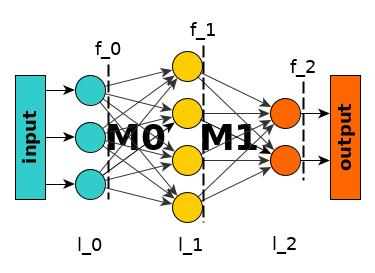
\includegraphics[scale=0.40]{layers.jpg}
\caption{Small neural network with layers $(l_0,l_1,l_2)$, weight matrix $(M_0,M_1)$ and activation functions $(f_0,f_1,f_2)$. Biases aren't represented for the sake of clarity.}
\label{layers}
\end{figure}

Neural networks are arranged in layers which communicate through weight matrices \ref{layers}. Layers are usually linear operations which means at the end of each layer a non linear function will be applied such as relu : 
$$ relu(x) = max(0,x) $$
This last one is particularly famous because it is easy to compute and performs well in practice.

\begin{equation*}
\begin{cases}
l_{i+1} = f_{i}(M_{i}. l_i + b_{i}) \\
l_0 = input \\
l_{q} = output
\end{cases}
\end{equation*}

with $l_{i}$ the $i^{th}$ layer ($i\le q$), $M_i$ the matrix to compute the excitatory signal leaving layer $l_{i}$ toward layer $l_{i+1}$, $f_i$ the activation function of layer $l_i$ (compute the activation of neurones from the excitatory signal) and $b_i$ is a bias.

The whole function is then $$out = f_q(M_q. ... f_i(M_i. ... f_0(M_0.input+b_0) ... + b_i) ... +b_q)$$ Parameters are matrix's weights and biases. They represent connection's strength between neurons and threshold to excited neurons. We'll see in next paragraph how to tune parameters to learn something to the neural network.

% je pense que toute la partie précédente avec les ANNs pourrait être plus claire, et plus step by step.  1. idée générale. 2. implémentation mathématique, pas à pas (e.g. comment est 1 neurone, puis comment ils sont connectés). Attention aussi de ne pas parler de choses que tu n'as pas expliquées auparavant, comme ici l'activation function. 
%-> I'd like to write something short. Writing 3 pages about neural networks isn't the point of my report so I'd like to keep it short and straightforward.
\paragraph{Supervised Learning}
In the supervised learning setting, a neural network learns to classify images using labeled data :
$$((x_0,y_0),(x_1,y_1), ... , (x_s,y_s))\in{\mathbb{R}^2}^s\indent(s\in\mathbb{N})$$
The goal is to make the neural neural fit on these values. This means that our model $f$ should verify $\forall i\le s, f(x_i) = y_i$ or at least $f(x_i) \approx y_i$. In practice the first case is almost impossible to reach and we try to minimize a \emph{loss function} that will define the '$\approx$' semantics. The simplest loss function is probably the squared L2 norm : $L = \sum_{i\le s}(f(x_i)-y_i)^2$.

To minimize this loss with a neural network we can compute the gradient of this loss for each parameter of the network and apply the gradient descent algorithm.
Gradient descent step :
$$\forall i\le n, w_i = w_i - \lambda  \frac{\partial L}{\partial w_i}$$
$$ \mbox{\emph{learning rate}} : 0<\lambda$$

If the gradient for a parameter $w$ is positive it means that the loss function should increase as the parameter increases. Thus by decreasing the value of this parameter the loss will decrease and the model will better fit the base. If it's negative the loss should decrease as the parameter increases.
By applying several steps of this algorithm it's possible for a neural network to approximate a base with a pretty good accuracy (L very low).

Defining the loss function is crucial as it will define the way gradients will be optimized which makes it one of the most important thing to work on in machine learning.


\subsubsection{Convolutional Neural Networks}
Convolutional neural networks are inspired by the internal structure of visual areas (LGN,V1,...) in brain. It makes it possible to compute images very efficiently. It's easier to understand convolutional neural networks by seeing states of layers as images (2 or 3D arrays) rather than a simple vector (1D array) as it was described previously.\newpage
\begin{figure}[!h]
\centering
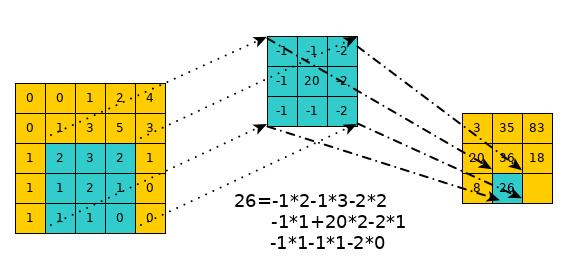
\includegraphics[scale=0.40]{conv.jpg}
\caption{Convolution computation}
\label{conv}
\end{figure}

\begin{figure}[!h]
\centering
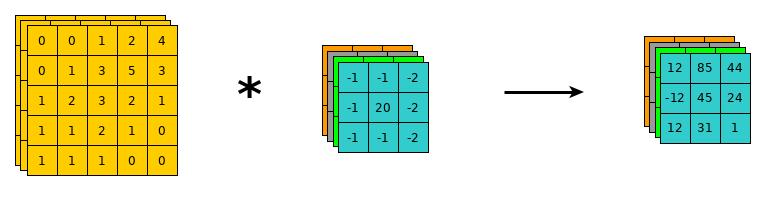
\includegraphics[scale=0.40]{conv2.jpg}
\caption{Convolution layer computation}
\label{conv2}
\end{figure}

Computation of a convolution with a kernel is represented in \ref{conv}. A convolution product is applied for each of the $c$ channels of the image and are then sumed to get a single channel image. This image is on of the channels of the output \ref{conv2}. Thus from an input with dimensions (h,w,c) and n kernels, the output has shape (h,w,n) (images are padded so that h and w doesn't vary).
Each layer has an internal matrix known as convolution kernel with few weights. This convolution product makes it possible to have a system invariant to translation which is particularly powerful when it comes to process images. 

The role of convolutions is to extract features from images : some kernels will catch straight lines where others might react more to circles. This way it makes it possible to extract more and more precises features from the images such as faces and specific textures.

However with only convolution layers, the shape of the image doesn't vary. It's very interesting to have more and more features as it is processed to have representations of many objects in order to classify them properly. That's why the number of channels must increase for deepest layers and the size of the image decrease as it makes it possible to have more focused features.

This is why people also use pooling layers combined with convolutions.

\begin{figure}[!h]
\centering
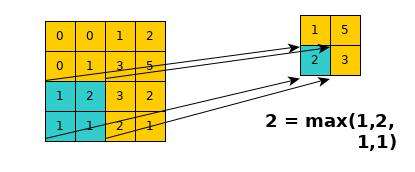
\includegraphics[scale=0.40]{pool.jpg}
\caption{Max Pooling layer computation}
\label{pool}
\end{figure}

Max Pooling layers reduce the size of the image as it goes through the network \ref{pool} by only keeping the sharpest details.

Usually people stack several convolutions, one pooling layer and a relu activation several times to make their network.

\subsubsection{Recurrent Neural Networks}
A recurrent neural network works similarly than a simple neural network excepts that it will keep an internal state that will interfer with next calls of the model.
\begin{equation*}
\begin{cases}
l_{i+1,t} = f_{i+1}(M_{i+1}. l_{i,t} + S_{i+1}.l_{i+1,t-1} + b_{i+1}) \\
l_{0,t} = input_t \\
l_{q,t} = output_t
\end{cases}
\end{equation*}
There is now a temporal system where the activation of the layer during the previous timestep is needed to compute timestep $t$. The first timestep is computed with an arbitrary value for the previous timestep (usually 0). This makes it possible for the network to remember previous information and to integrate information through time. Gradient descent works similarly by backpropagating through timesteps. However the network might forget rather quickly the first timesteps when the training is long (high number of timesteps).

That's why there are many variants for the way to use the internal state of recurrent networks, such as LSTM (Long Short Term Memory) that will make it possible for the network to control which parts of the internal state to remember or discard.


%I'll probably change this part. It's not very clear
\subsection{Reinforcement Learning}
Reinforcement learning involves an agent / environment system where the agent will have to learn to behave in order to maximize a reward.

More formally the environment contains a set of states $S$, a set of initial states $S_I\in S$, a set of final states $S_f \in S$, a finite set of actions that can be taken in any state $A$, a stochastic transition function $P$ being a probability distribution over events $S$ ($P(S_{i+1}|S_i,A_i$) reprensents the probability when taking an action $A_i$ in state $S_i$ that the environment goes in state $S_{i+1}$ )and a reward function $R$:($S$,$A$)$\rightarrow\mathbb{R}$ telling which reward is associated with a transition. This is part of the environment, the agent doesn't know $S$,$A$,$P$ nor $R$ and will explore them.

A trajectory in the environment is a finite run from an initial state to a final state : $(S_0,A_0,R_0),...,(S_i,A_i,R_i),...,(S_q,A_q,R_q)$. The final state is often excluded of the trajectory as no action is taken in it. Trajectory must be admissible ($\forall i\le n,P(S_{i+1}|S_i,A_i) > 0$). The set of trajectories will be called $T$. Trajectories might be infinite if the environment allows it but in practice they are finite.

Initially the agent jumps in the environment with 0 knowledge about it and it will have to explore to learn where best rewards are and which trajectories in $P$ are the most interesting ones. It will have a memory $M$ that is the set of previous trajectories in the environment. The agent behaviour will be modelised by a function $\pi$:$(S,\mathbb{P}(T))\rightarrow [0,1]^A$ called the \emph{policy} associating a probability distribution over the action space to each state and memory. This function will be learnt.

Each step, the agent is in a state $S_i$ and chooses an action $A_{i} = \pi(S_i\|M+((S_0,A_,R_0),...,(S_{i-1},A_{i-1},R_{i-1})))$ which changes its state to $S_{i+1}=T(S_i,A_i)$ and returns the reward $R_i$= $R$($S_i$,$A_i$). If the new state is final, the trajectory is over, if it's not, the agent continues to step. Initially the agents starts in an initial state $S_0$ (chosen arbitrarily of randomly) and steps.

We can define a \emph{return} over a trajectory as the sum of rewards for this trajectory. However in most cases it is more interesting to use a discounted sum of rewards as it gives an idea of neighbourhood to the gain function:
$$ R_{\pi}(\tau) = \sum_{(S_i,A_i,R_i)\in\tau}\gamma^{i}.R_i $$
$$ \gamma \in ]0,1[$$
This quantity defines the reward obtained over trajectory $\tau$ by following policy $\pi$ ($\pi$ isn't used in the computation, it's just for notations : this \emph{return} represents reliability of $\pi$).


To improve the agent will run several trajectories always trying to understand better its environment and finding the best policy to optimize its gain. After each trajectory $\pi$ might be updated by the RL algorithm for this purpose.

The aim of RL is to find the best algorithm to maximize the sum of gain only giving the agent a specified period of time to improve. In practice it could be a robot trying to find a path in ruins of a collapsed building to find survivors. It needs to understand in real time the shape of the environment to map it and to avoid getting hurt. This means it will very often have to choose between exploring of exploiting what the agent already knows. If it explores all the time it won't be able to get enough reward especially if time is short whereas if it explores a bit and after only exploits it knowledge without learning more it may get far less reward than it could.

In practice it's almost impossible to get a complete understanding of the environment (think about Chess and Go which are too complex games with too many states / actions to be fully explored). This means the policy needs to extrapolate its knowledge understanding a logics behind the environment. This can be acheived using tools such as Neural Networks. There are many ways to optimize $\pi$ function but to make it short we will only explore the Policy Gradient method.

In practice observation space and action space are arrays of float values.

In RL there are 2 additional usefull functions that will be used later : $Q$ and $V$. 
$$\forall s\in S, Q_\pi(s,a)=\mathbb{E}_{\tau\|\tau[0]=(s,a,\_)}(R_\pi(\tau)) $$
$$\forall (s,a)\in S\times A, V_\pi(s)=\mathbb{E}_{\tau\|\tau[0]=(s,\_,\_)}(R_\pi(\tau)) $$
$Q_\pi$ represents the value of an action in a specific state after taking this action with policy $\pi$ whereas V represents the value of a state while following $\pi$. We then finaly define optimal $V$ and $Q$ :
$$\forall s\in S,V_*(s) = max_\pi V_\pi(s)$$
$$\forall (s,a)\in S\times A,Q_*(s,a) = max_\pi Q_\pi(s,a)$$



\subsubsection{Policy Gradient - REINFORCE}
The philosophy of policy gradient methods is to see the policy $\pi$ as a function that will be learnt by supervised learning on batches of observations.  The aim of policy gradient is to use a neural network as policy model and to use a specific loss function to increase the score of the agent. This policy will have a probability of chosing a random action as exploration parameter instead of returning its estimated best action.

Usually the algorithm will proceed in 2 phases : first it will collect information from the environment (n trajectories) and then it will fit the policy on those collected data. The policy will be modelised by a neural network which will, given an observation (a vector), return the associated action (a vector).

REINFORCE is probably the simplest Policy Gradient algorithm and is directly using the sum of the estimated expectation over the batch of collected data as loss for the neural network.
$$-\mathbb{E}(\sum_{\tau}R_{\pi}(\tau))$$
The algorithm collects a batch of X trajectories to fit the neural network on it. This process is repeated several time until convergence.
% I don't know if I explain in depth why it's easily computable and independant from P because it might be a lot of math but it helps understanding how it works
This function can be easily computed in practice as well as its gradient especially because the gradient only depends on the policy and not on $\pi$. This process of collecting / fitting is repeated several times.



\subsubsection{PPO}
PPO is a state of the art Policy Gradient algorithm designed by OPENAI. It aims at improving REINFORCE by adding few features in the loss function. First when using an algorithm such as REINFORCE, the policy might change too much when fitting. Let's assume the environment is divided into several phases (summer,automn,winter,spring for example) where results of actions could be very different from a phase to another. This kind of learning might result in a policy that would change too much and overfit on each phase, forgetting everything learnt during the previous phase. There is no perfect solution for this issue.

PPO adds a term in the loss that will try to not move too much from the previous policy in order to avoid such a behaviour. This term uses a more complex structure than REINFORCE. The policy will be composed of 2 neural networks : the policy network which returns actions and the value network. Both uses the same input and that's why very often they form a single network with 2 outputs : the action vector (policy network) and an additional output (float) for the value network. The role of the value network is to estimate the value of the actual state ($V(s)$ we have discussed about earlier). We can then define the \emph{advantage function} as $\hat A_{\pi}(s,a)$ = $Q_\pi(s,a)-V_\pi(s)$. It represents the interest of taking action $a$ in state $s$ rather than $a'$. If it's positive it means that $a$ is better than the average.

Finally we need a last definition : $\hat r_{\pi,\pi_{old}}(s,a) = \frac{\pi(a|s)}{\pi_{old}(a|s)}$ the ratio between actual policy and the previous one. This ratio quantifies movements in the policy and this term will allow the loss to minimize them as well as improving the policy. This trade-off between both stabilizes the learning. We can finally define the PPO loss :
$$L_{clip} = \mathbb{E}(\sum_{(s_i,a_i,r_i)\in\tau}(\min(\hat r_{\pi,\pi_{old}}(s_i,a_i)\hat A_t,clip(\hat r_{\pi,\pi_{old}}(s_i,a_i),1-\epsilon,1+\epsilon)\hat A_t)))$$
It's a very complex loss that will be maximized instead of minimized. To understand what it does let's consider the inner term :
$$\min(\hat r_{\pi,\pi_{old}}(s_i,a_i)\hat A_t,clip(\hat r_{\pi,\pi_{old}}(s_i,a_i),1-\epsilon,1+\epsilon)\hat A_t)$$
The first part is 
$$\hat r_{\pi,\pi_{old}}(s_i,a_i)\hat A_t$$
If $\hat A_t$ is positive, then the action that has been taken is better than expected which means its probability should be increased. By increasing the loss, $\hat r_{\pi,\pi_{old}}(s_i,a_i)$ will increase which means the probability for $a_i$ to be taken in $s_i$ will tend to be more likely than in previous policy.

Now let's take a look at the other term :
$$clip(\hat r_{\pi,\pi_{old}}(s_i,a_i),1-\epsilon,1+\epsilon)\hat A_t)$$
This clipping makes it possible for the loss to stay constant if $\hat r_{\pi,\pi_{old}}$ is too far from 1.

\begin{figure}[!h]
\centering
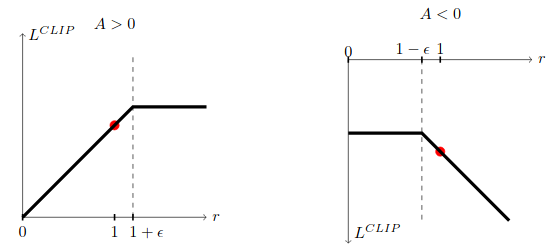
\includegraphics[scale=0.40]{curve_ppo.png}
\caption{PPO inner term}
\label{ppo_curve}
\end{figure}

This means that it will flatten the curve of the loss  in order to prevent the algorithm to try to go too far from previous policy. The min operator will then ensure the continuity of curves \ref{ppo_curve}.


This algorithm has proven very efficient lately.

\end{document}
